\section{ТЕОРЕТИЧЕСКИЕ СВЕДЕНИЯ}

Семантическая сеть состоит из вершин различных типов.
В простейшем случае различают вершины-объекты и вершины отношения.
Рассмотрим предложение: <<Петр читает газету>>.
Здесь имеется два объекта (Петр, газета) и отношение (читает),
которое, как правило, передается глаголом.
Это замечание имеет универсальный характер.
Объекты предметного мира вступают в различные отношения, передаваемые глаголами.
Данную фразу можно представить графически,
как показано на рисунке~\ref{fig:sem_network}.

\begin{figure}[h!]
  \centering
  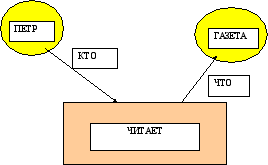
\includegraphics[width=120mm]{img/sem_network}
  \caption{Пример семантической сети}
  \label{fig:sem_network}
\end{figure}

Слова <<кто>> и <<что>> над стрелками задают так называемые
падежные отношения.
Из такого представления ясно, кто выступает носителем
(субъектом) действия, кто (что) является объектом действия и
каково само действие.

\newpage